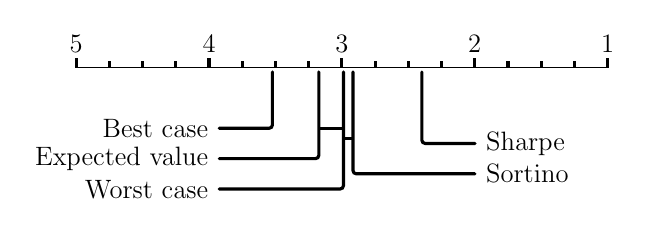
\begin{tikzpicture}[
  treatment line/.style={rounded corners=1.5pt, line cap=round, shorten >=1pt, line width=.5mm},
  treatment label/.style={font=\large},
  group line/.style={ultra thick},
  scale={0.8},
]

\begin{axis}[
  clip={false},
  axis x line={center},
  axis y line={none},
  axis line style={-},
  xmin={1},
  ymax={0},
  scale only axis={true},
  width={\axisdefaultwidth},
  ticklabel style={anchor=south, yshift=1.3*\pgfkeysvalueof{/pgfplots/major tick length}, font=\large},
  every tick/.style={draw=black, line width=.5mm},
  major tick style={yshift=.5*\pgfkeysvalueof{/pgfplots/major tick length}},
  minor tick style={yshift=.5*\pgfkeysvalueof{/pgfplots/minor tick length}},
  title style={yshift=\baselineskip},
  xmax={5},
  ymin={-3.5},
  height={4\baselineskip},
  xtick={1,2,3,4,5},
  minor x tick num={3},
  x dir={reverse},
]

\draw[treatment line] ([yshift=-2pt] axis cs:2.3981481481481484, 0) |- (axis cs:1.9814814814814816, -2.5)
  node[treatment label, anchor=west] {Sharpe};
\draw[treatment line] ([yshift=-2pt] axis cs:2.9166666666666665, 0) |- (axis cs:1.9814814814814816, -3.5)
  node[treatment label, anchor=west] {Sortino};
\draw[treatment line] ([yshift=-2pt] axis cs:2.988425925925926, 0) |- (axis cs:3.939814814814815, -4.0)
  node[treatment label, anchor=east] {Worst case};
\draw[treatment line] ([yshift=-2pt] axis cs:3.173611111111111, 0) |- (axis cs:3.939814814814815, -3.0)
  node[treatment label, anchor=east] {Expected value};
\draw[treatment line] ([yshift=-2pt] axis cs:3.5231481481481484, 0) |- (axis cs:3.939814814814815, -2.0)
  node[treatment label, anchor=east] {Best case};
\draw[group line] (axis cs:2.9166666666666665, -2.3333333333333335) -- (axis cs:2.988425925925926, -2.3333333333333335);
\draw[group line] (axis cs:2.988425925925926, -2.0) -- (axis cs:3.173611111111111, -2.0);

\end{axis}
\end{tikzpicture}